\section{TP: Revivons les grands frissons d'une éruption solaire}

Les principales éruptions solaires sont listées sur la page \url{http://en.wikipedia.org/wiki/Solar_cycle_24}.

\subsection{Introduction}

Le but de ce TP est de construire une vidéo à partir de données collectées sur le soleil par le \emph{Solar Dynamics Observatory}\footnote{http://aia.lmsal.com/index.htm}. On utilisera uniquement les images du soleil capturées à intervalle régulier. Les images sont disponibles à l'adresse \url{http://jsoc.stanford.edu/data/aia/images/}. Elles sont classées par date de mesure, la structure du répertoire distant étant~:
\begin{center}
http://jsoc.stanford.edu/data/aia/images/YYYY/MM/DD/$\lambda$/fichier.jp2
\end{center}

Le SDO observe le soleil dans différentes longueurs d'onde $\lambda \in [\mathlist{94\si{\AA}, 131\si{\AA}, 171 \si{\AA}, 193\si{\AA}, 211\si{\AA}, 304\si{\AA}, 335\si{\AA}, 1600\si{\AA}, 1700\si{\AA}, 4500\si{\AA}}]$. Pour avoir une idée des mesures à ces différentes longueurs d'onde, vous pouvez vous rendre à l'adresse \url{http://sdo.gsfc.nasa.gov/data/}, ou bien regarder l'image ci-dessous. On trouvera une description de ce qui est observé à ces différentes longueurs d'onde sur le site de la Nasa \url{http://www.nasa.gov/mission_pages/sunearth/news/light-wavelengths.html}.
\begin{figure}[htbp]
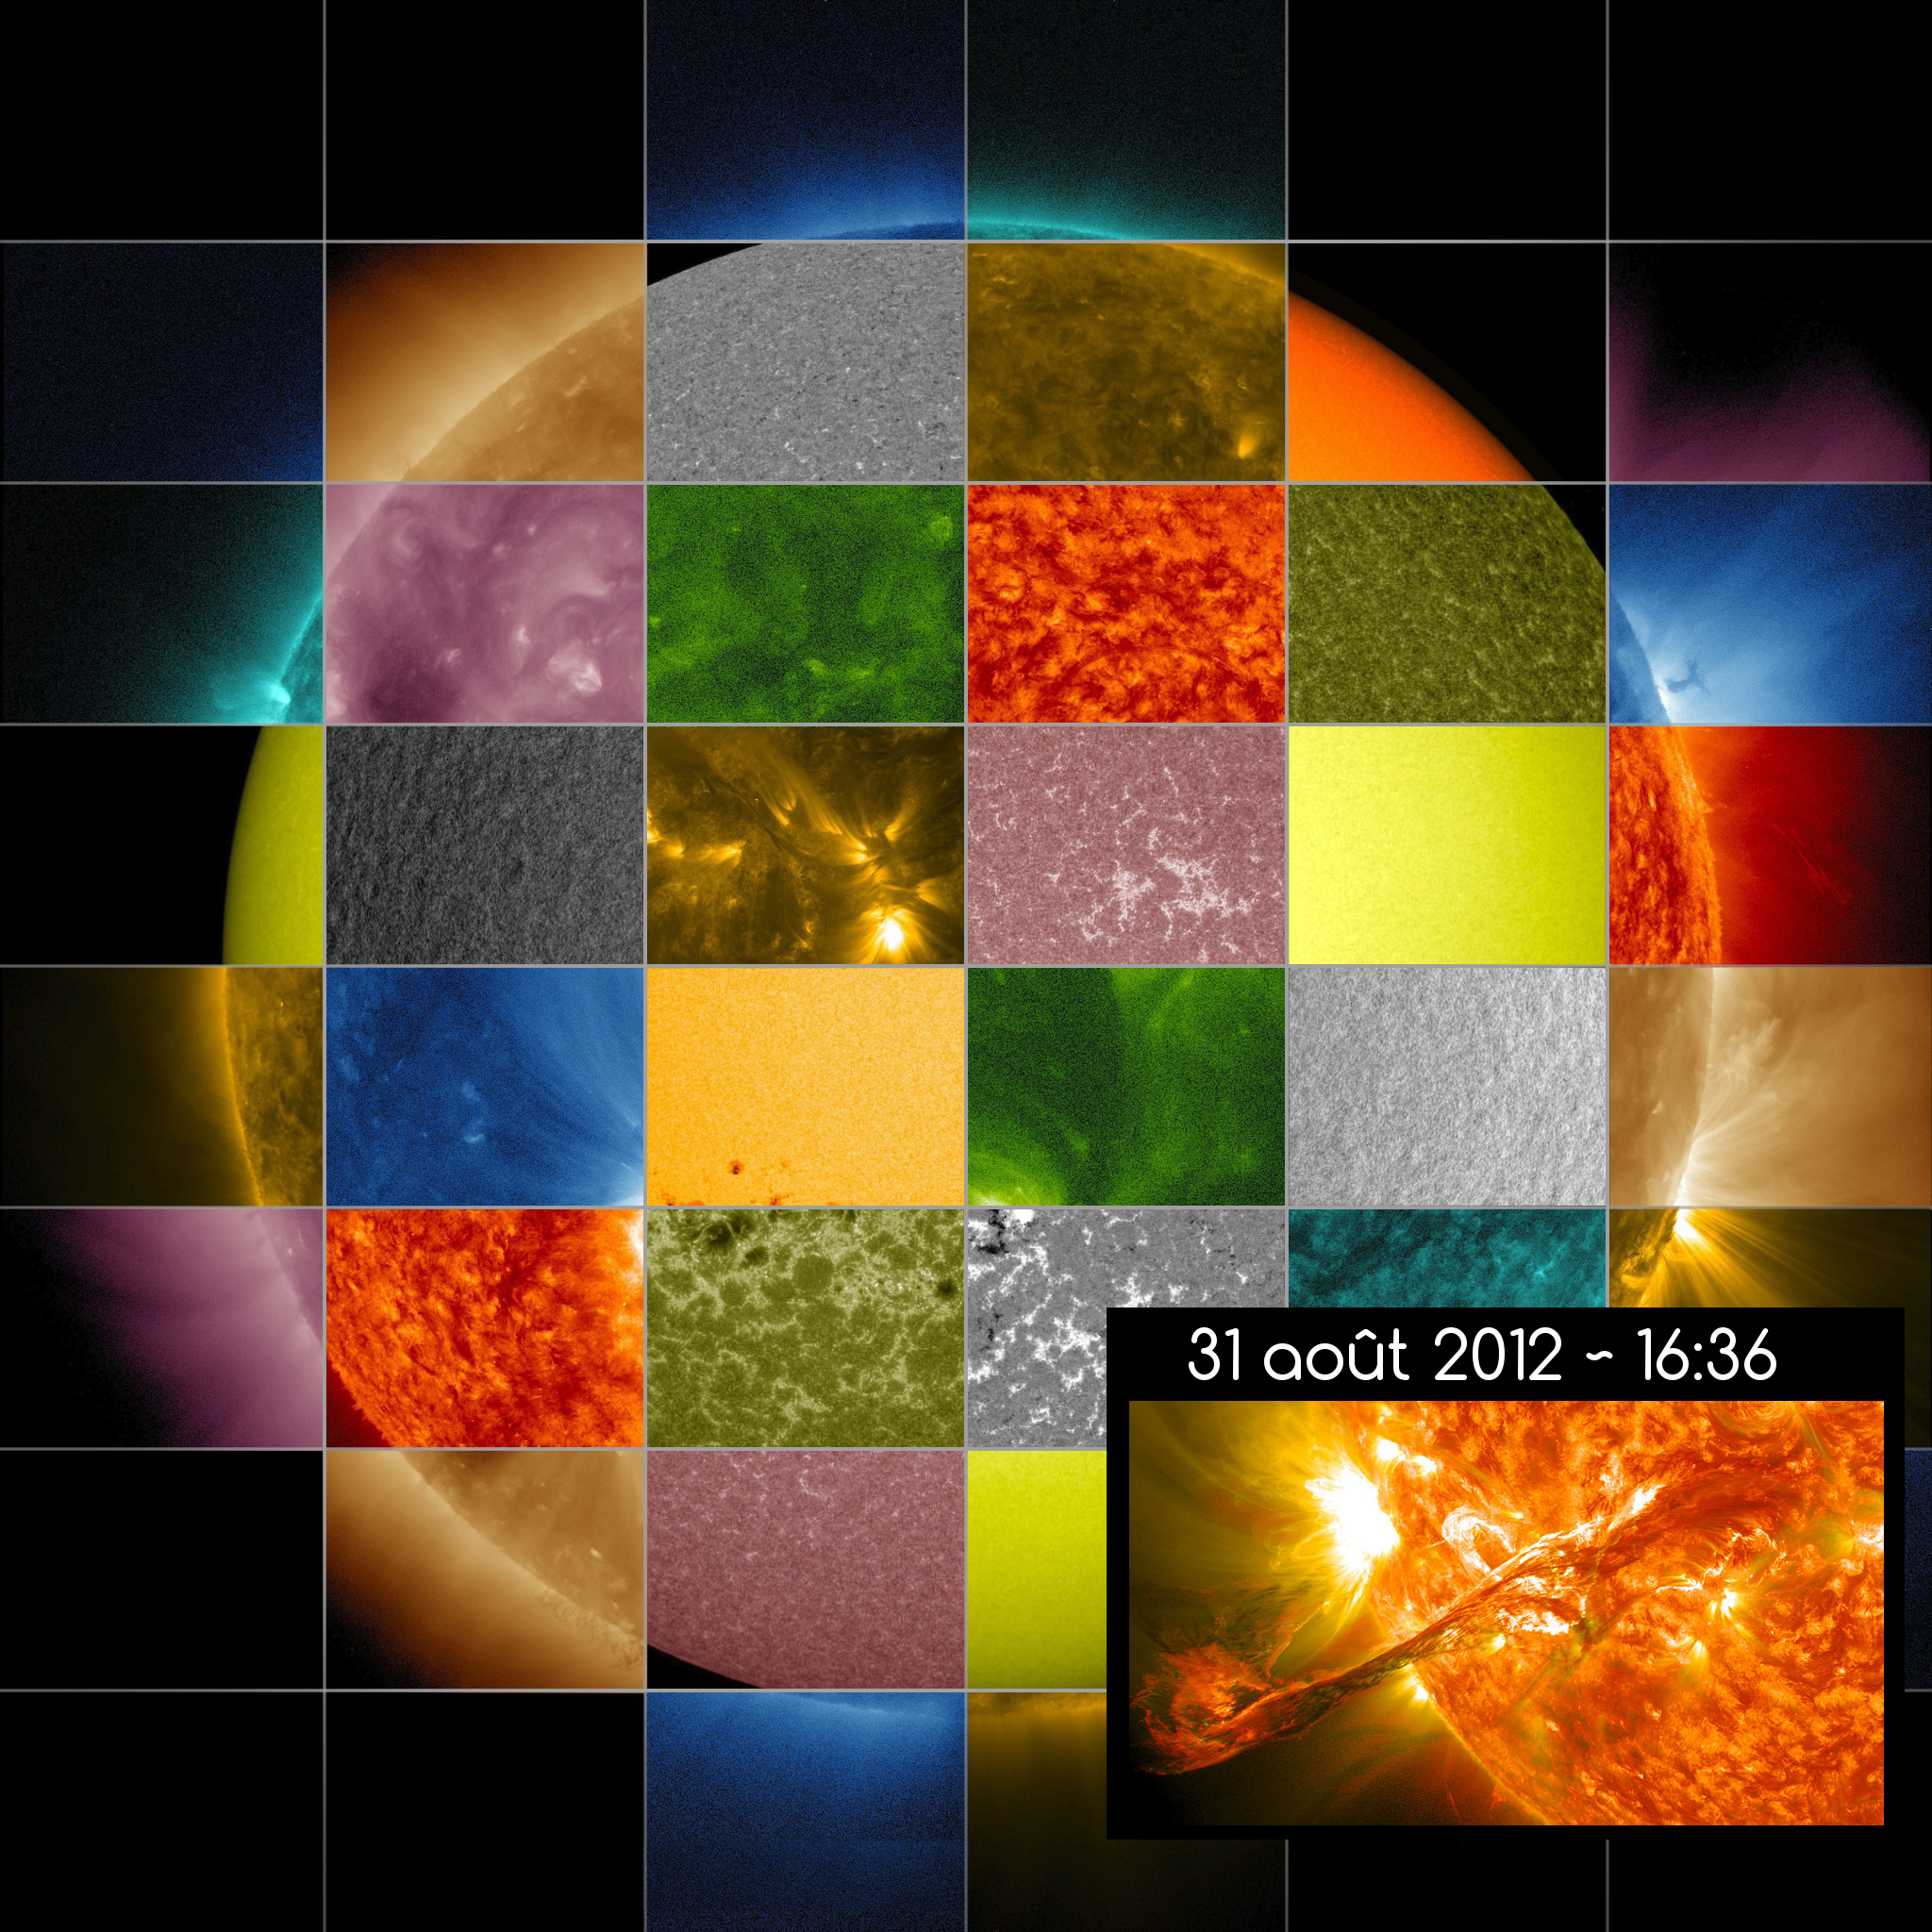
\includegraphics[width=0.65\linewidth]{Figs/solar_wavelength2.jpg}
\end{figure}

Durant ce TP, je vous propose d'utiliser les mesures à $211 \si{\AA}$. Les images sont au format JPEG2000 avec l'extension $jp2$ et une résolution de $4096 \times 4096$. Dans ce TP, on cherche à illustrer la construction de programmes du type ``puits | commande1 | commande2 ....''. On va récupérer les images, les convertir en JPEG, les redimensionner, y incruster la date et l'heure de la mesure et les combiner pour construire une vidéo. On va voir dans ce TP l'utilisation d'un certain nombre de programmes tels que \bashcmd, \wget, \convert (imagemagick), \gawk, \sed et \ffmpeg. On cherche ainsi à ne pas réinventer la roue, votre problème est de produire une vidéo à partir des images brutes et on va voir qu'en assemblant plusieurs briques déjà existantes, on peut facilement résoudre ce problème.

\begin{center}
\colorbox{lblue}{\begin{minipage}{\linewidth}

\includegraphics[width=0.05\columnwidth]{Figs/warning.png}
\includegraphics[width=0.05\columnwidth]{Figs/warning.png}
\textbf{Attention}: Dans tout ce qui suit, on remplacera le préfixe des adresses web http://jsoc.stanford.edu/ par http://infomob/fix/. Sur http://infomob.metz.supelec.fr/fix/ on retrouvera plusieurs jeux d'images que j'ai récupéré de leurs serveurs, à savoir~:
\begin{itemize}
\item le 07/06/2011 en $304\si{\AA}$ : grosse éruption entre 6h et 7h
\item le 31/08/2012 en $211\si{\AA}$ et $171\si{\AA}$ : petite éruption autour de 19:00
\end{itemize}
Il y a plusieurs raisons à l'utilisation de ce miroir local: 1) les temps d'accès, 2) je crains que si tout le monde accède de manière répétée au site jsoc.stanford.edu, nous soyons banis de leur serveur web et donc qu'on ne puisse pas faire correctement le TP, 3) on ne surcharge pas inutilement leurs serveurs pour nos TPs.
\end{minipage}}
\end{center}


\subsection{Structure du projet}

Je vous propose de créer quelques répertoires pour structurer votre projet. Pour les créer, forcez vous à utiliser les commandes \mkdir, \ls, etc.. depuis un terminal.
\begin{itemize}
\item scripts : contiendra la plupart des scripts que vous écrirez,
\item raw\_images : contiendra de manière temporaire les images brutes au format .jp2,
\item images: contiendra les images converties au format jpeg et redimensionnées,
\item postproc\_images: contiendra les images jpeg dans lesquelles la date et l'heure auront été incrustées
\item video : contiendra les vidéos générées
\end{itemize}

La figure \ref{fig:soleil_overview} donne une vision d'ensemble du programme que nous allons écrire.

\begin{center}
\begin{figure}
\begin{tikzpicture}[
  font=\sffamily,
  every matrix/.style={ampersand replacement=\&,column sep=2cm,row sep=2cm},
  source/.style={draw,thick,rounded corners,fill=blue!20,inner sep=.3cm},
  datastore/.style={draw,very thick,shape=datastore,inner sep=.3cm},
  command/.style={draw,dashed, rounded corners,fill=yellow!30,inner sep=.3cm},
  dots/.style={gray,scale=2},
  to/.style={->,>=stealth',shorten >=1pt,semithick,font=\sffamily\footnotesize},
  todash/.style={->,>=stealth',shorten >=1pt,dashed,semithick,font=\sffamily\footnotesize},
  every node/.style={align=center}]

  % Position the nodes using a matrix layout
  \matrix{
    \node[source] (commande) {31/08/2012, $211 \si{\AA}$};
      \& \node[datastore] (getindex) {get\_index.sh}; 
      \& \node[command] {lynx, more, (mktemp)};\\

    \& \node[datastore] (extract) {extract\_url.sh}; 
      \& \node[command] {gawk};\\

     \& \node[datastore] (telecharge) {telecharge\_img.sh}; 
      \& \node[command] {wget};\\

     \& \node[datastore] (convert) {convert\_img.sh}; 
      \& \node[command] {convert, rm};\\

     \& \node[datastore] (date) {ecrit\_date.sh}; 
      \& \node[command] {sed, convert};\\

     \node[source] (resultat) {31\_08\_2012\_211.mp4};
     \& \node[datastore] (video) {creer\_video.sh}; 
      \& \node[command] {ffmpeg};\\    
  };

  % Draw the arrows between the nodes and label them.
  \draw[to] (commande) -- (getindex);
  \draw[to] (getindex) -- node[midway,right] {contenu de \\ http://jsoc.../2012/08/31/211/} (extract);
  \draw[to] (extract) --  node[midway,right] {URL des images \\http://jscoc.stanford..../2012\_08\_31\_\_00....jp2\\............\\ http://jscoc.stanford..../2012\_08\_31\_\_23....jp2} (telecharge);
  \draw[to] (telecharge) --  node[midway,right] {Images brutes\\./raw\_images/2012\_08\_31\_\_00....jp2\\............\\./raw\_images/2012\_08\_31\_\_23....jp2} (convert);
  \draw[to] (convert) -- node[midway,right] {Images converties et redimensionnées\\./images/2012\_08\_31\_\_00....jpg\\............\\./images/2012\_08\_31\_\_23....jpg} (date);
  \draw[todash] (date) -- node[midway,right] {Images renommées, avec date et heure\\./postproc\_images/00000.jpg\\............\\./postproc\_images/02479.jpg}(video);
  \draw[to] (video) -- (resultat);
  %% \draw[to] (buffer) --
  %%     node[midway,right] {raw event data\\level 1} (monitor);
  %% \draw[to] (monitor) to[bend right=50] node[midway,above] {events}
  %%     node[midway,below] {level 1} (storage);
  %% \draw[to] (storage) to[bend right=50] node[midway,above] {events}
  %%     node[midway,below] {level 1} (monitor);
  %% \draw[to] (monitor) -- node[midway,above] {events}
  %%     node[midway,below] {level 1} (datastore);
\end{tikzpicture}
\caption{Vue d'ensemble du TP ``Revivons les grands frissons d'une éruption solaire''.\label{fig:soleil_overview}}
\end{figure}
\end{center}

\subsection{Récupération des données d'une journée}

Le but de cette partie est d'écrire un script Bash qui se charge de récupérer les images d'une journée. Ce script prendra 4 arguments, à savoir l'année YYYY, le mois MM, le jour DD et la longueur d'onde $\lambda$ des mesures. Il devra produire en sortie le flux des URLs des images de cette journée particulière à la longueur d'onde $\lambda$.\\

Si vous allez sur le site \urlsoleil, et regardez les images du \datesoleil, vous constaterez qu'il y a énormément d'images, prises à des heures régulières mais dont on ne peut pas facilement prédire le nom de fichier. On va donc procéder différemment: on va lister l'ensemble des images disponibles dans le répertoire du \datesoleil à \lambdasoleil. Pour cela, on va utiliser l'explorateur \lynx (n'hésitez pas à appeler man lynx pour en savoir plus). \lynx est un explorateur internet textuel, sans fenêtre graphique, qui s'affiche dans la console.\\

\textbf{Lancez} \lynx et décortiquez l'interface pour effectuer une recherche de votre choix sur google.\\

Je suis d'accord avec vous, cette manière d'explorer internet n'est pas très confortable. Mais, on peut utiliser \lynx pour récupérer le contenu d'une page grâce à l'option dump 'lynx -dump URL'. En ajoutant l'option '-listonly', on ne récupère que la liste des références (les liens vers les images dans notre cas). Essayez la commande ci-dessous:
\begin{center}
\bash{lynx -dump -listonly http://jsoc.stanford.edu/data/aia/images/2012/08/31/211/ | less }
\end{center}
Il apparaît le contenu de la page, converti en texte, dans lequel vous pouvez naviguer avec les flèches directionnelles. Le contenu affiché devrait ressembler à ça~:
\begin{exempleResultat}
Références

   1. http://jsoc.stanford.edu/data/aia/images/2012/08/31/211/?C=N;O=D
   2. http://jsoc.stanford.edu/data/aia/images/2012/08/31/211/?C=M;O=A
   3. http://jsoc.stanford.edu/data/aia/images/2012/08/31/211/?C=S;O=A
   4. http://jsoc.stanford.edu/data/aia/images/2012/08/31/211/?C=D;O=A
   5. http://jsoc.stanford.edu/data/aia/images/2013/05/01/
   6. http://jsoc.stanford.edu/data/aia/images/2012/08/31/211/2012\_08\_31\_\_00\_00\_23\_34.jp2
   7. http://jsoc.stanford.edu/data/aia/images/2012/08/31/211/2012\_08\_31\_\_00\_00\_59\_34.jp2
   8. http://jsoc.stanford.edu/data/aia/images/2012/08/31/211/2012\_08\_31\_\_00\_01\_35\_34.jp2
   9. http://jsoc.stanford.edu/data/aia/images/2012/08/31/211/2012\_08\_31\_\_00\_02\_11\_34.jp2
  10. http://jsoc.stanford.edu/data/aia/images/2012/08/31/211/2012\_08\_31\_\_00\_02\_47\_34.jp2
  11. http://jsoc.stanford.edu/data/aia/images/2012/08/31/211/2012\_08\_31\_\_00\_03\_23\_34.jp2
  12. http://jsoc.stanford.edu/data/aia/images/2012/08/31/211/2012\_08\_31\_\_00\_03\_59\_34.jp2
  13. http://jsoc.stanford.edu/data/aia/images/2012/08/31/211/2012\_08\_31\_\_00\_04\_35\_34.jp2
 \end{exempleResultat}

Notez qu'on a redirigé la sortie standard de \lynx dans l'entrée standard de \less. \less est un programme qui permet de parcourir du contenu texte (e.g. un fichier mais il peut également lire depuis l'entrée standard).\\


\textbf{Écrivez} un script bash $scripts/get\_index.sh$ qui~:
\begin{itemize}
\item prenne le jour, le mois, l'année et la longueur d'onde des mesures à récupérer
\item récupère le contenu de la page grâce à lynx -dump -listonly 
%\item redirige dans la sortie standard le contenu téléchargé (on pourra utiliser le programme \cat pour afficher dans la sortie standard le contenu d'un fichier)
\end{itemize}

\subsection{Extraire les URLs des images}

Le contenu affiché par le script précédent contient beaucoup d'informations. On souhaite en extraire les URLs vers les images listées sur la page. Les URLs que nous cherchons à extraire ont un format très particulier; elles commencent par "http://"  et finissent par ".jp2". Pour filtrer les lignes qui ne contiennent que ce motif, on va utiliser \gawk et ce qu'on appelle des expressions régulières.\\

\awk est un programme qui applique un programme sur un fichier (ou l'entrée standard) ligne par ligne. Un programme awk est de la forme 'pattern \{ action \}'. \awk comprends ce mini-programme comme ``si la ligne est filtrée par le patron \emph{pattern} alors on réalise l'action \emph{action}'. Par ailleurs, \awk divise la ligne selon un séparateur (modifiable par l'option '-FS ``sep'''), qui est l'espace ' ' par défaut.\\

Prenons un exemple concret. Exécutez votre script get\_index.sh et redirigez la sortie standard dans un fichier~:
\begin{exempleResultat}
bash:\$ ./scripts/get\_index.sh 31 08 2012 211 > 31\_08\_2012\_211
bash:\$ less 31\_08\_2012\_211
\end{exempleResultat}
 
On y retrouve bien la liste des liens vers les images du \datesoleil. On va maintenant lire le fichier avec \cat et le faire passer par \awk.
\begin{exempleResultat}
bash:\$ cat 31\_08\_2012\_211 | awk '\{ print \$0 \}'
bash:\$ cat 31\_08\_2012\_211 | awk '\{ print \$1 \}'
bash:\$ cat 31\_08\_2012\_211 | awk '\{ print \$2 \}'
\end{exempleResultat}

Si vous voulez voir plus en détails la sortie de awk, n'hésitez pas à rediriger sa sortie dans less en ajoutant '| less'. Les \emph{pattern} et \emph{action} de programme \awk peuvent prendre plusieurs formes (voir \url{http://www.gnu.org/software/gawk/manual/gawk.html#Patterns-and-Actions}), on ne va en voir ici que certaines d'entre elles.  Dans l'exemple ci-dessus, nous n'avons pas précisé de \emph{pattern}, toutes les lignes sont ainsi retenues et vous avez dû constaté que la première commande affiche toute la ligne, la deuxième seulement le numéro du lien et la dernière l'adresse. Quand \awk parcours une ligne, il crée plusieurs variables utilisables dans les \emph{pattern} et \emph{action}, en particulier les variables \$0, \$1, ... \$NF qui permettent d'accéder aux champs extraits par \awk (\url{http://www.gnu.org/software/gawk/manual/gawk.html#Fields}). \$0 est une variable particulière qui contient toute la ligne lue par \awk. Les champs sont accessibles par les variables \$1, \$2, ... ; Il y a également d'autres variables, comme NF égal au nombre de champs dans la ligne, de telle sorte que \$NF sera toujours le dernier champ extrait. La variable NR contient le numéro de ligne lu, ... \\

A titre d'exemple, on peut facilement décoder la lettre envoyée par George Sand à Alfred de Musset ci-dessous~:
\begin{center}
\begin{verbatim}
Cher ami,
Je suis toute émue de vous dire que j'ai
bien compris l'autre jour que vous aviez
toujours une envie folle de me faire
danser. Je garde le souvenir de votre
baiser et je voudrais bien que ce soit
une preuve que je puisse être aimée
par vous. Je suis prête à montrer mon
affection toute désintéressée et sans cal-
cul, et si vous voulez me voir ainsi
vous dévoiler, sans artifice, mon âme
toute nue, daignez me faire visite,
nous causerons et en amis franchement
je vous prouverai que je suis la femme
sincère, capable de vous offrir l'affection
la plus profonde, comme la plus étroite
amitié, en un mot : la meilleure épouse
dont vous puissiez rêver. Puisque votre>
âme est libre, pensez que l'abandon ou je
vis est bien long, bien dur et souvent bien>
insupportable. Mon chagrin est trop
gros. Accourrez bien vite et venez me le
faire oublier. À vous je veux me sou-
mettre entièrement.
Votre poupée 
\end{verbatim}
\end{center}

en utilisant la commande awk : \bash{awk 'NR \% 2 == 1 \{ print \$0 \}'} qui permet d'afficher toutes les lignes d'indice impair. La réponse de Musset ci-dessous~:

\begin{center}
\begin{verbatim}
Quand je mets à vos pieds un éternel hommage,
Voulez-vous qu'un instant je change de visage ?
Vous avez capturé les sentiments d'un coeur
Que pour vous adorer forma le créateur.
Je vous chéris, amour, et ma plume en délire
Couche sur le papier ce que je n'ose dire.
Avec soin de mes vers lisez les premiers mots,
Vous saurez quel remède apporter à mes maux. 
\end{verbatim}
\end{center}

se décrypte facilement en utilisant awk. Le programme decode\_musset.awk ci-dessous permet en effet de le décrypter \bash{awk -f decode\_musset.awk musset\_sand.txt}. Dans le programme AWK, ORS signifie ``Output Record Separator'' c'est à dire le caractère utilisé entre chaque résultat filtré.

\begin{verbatim}
BEGIN { ORS = " " } 
{ print $1 }
END { print "? \n" }
\end{verbatim}

Le premier exemple utilise une expression arithmétique (\bash{NR \% 2 == 1}) comme \emph{pattern}. On peut également utiliser des expressions régulières. Par exemple, pour vérifier si une ligne contient une URL vers une image au format jp2, on peut utiliser la commande awk~: \bash{awk '/http:\textbackslash{}/\textbackslash{}/.*\textbackslash{}.jp2/ \{ print \$2 \}'}. Cette commande un peu étrange recherche, dans la ligne courante, une chaîne de caractère de la forme http:// (\bash{http:\textbackslash{}/\textbackslash{}/}), suivi d'un nombre arbitraire de caractères (\bash{.*}), suivi de .jp2 (\bash{\textbackslash{}.jp2}). Si cette expression régulière est vérifiée, alors le deuxième champs \$2 est affiché. \textbf{Ecrivez un script} bash \bash{scripts/extract\_url.sh} qui, étant donné la liste des références obtenues avec Lynx, produise un flux dans la sortie standard des URL des images.\\

\textbf{Testez le script} que vous venez d'écrire en lui donnant en entrée un contenu récupéré par Lynx. Je vous propose d'utiliser le fichier 2012\_08\_31\_211 que avez créé précédemment. Pour lire ce fichier et le rediriger vers l'entrée standard, nous utilisons la commande \bash{cat}. Vous pouvez donc vérifier le fonctionnement de votre script par la commande ci-dessous~:
\begin{center}
\bash{cat 31\_08\_2012\_211 | ./scripts/extract\_url.sh}
\end{center}
Cela devrait vous afficher les URLs de toutes les images. Pour n'en afficher qu'une partie, par exemple les 10 premières ou 10 dernières, vous pouvez utiliser les commandes \bash{head} et \bash{tail}~:
\begin{center}
\bash{cat 31\_08\_2012\_211 | ./scripts/extract\_url.sh | head -10}
\end{center}
Ce qui devrait produire~:
\begin{exempleResultat}
http://jsoc.stanford.edu/data/aia/images/2012/08/31/211/2012_08_31__00_00_11_63__SDO_AIA_AIA_211.jp2
http://jsoc.stanford.edu/data/aia/images/2012/08/31/211/2012_08_31__00_00_47_62__SDO_AIA_AIA_211.jp2
http://jsoc.stanford.edu/data/aia/images/2012/08/31/211/2012_08_31__00_01_23_62__SDO_AIA_AIA_211.jp2
http://jsoc.stanford.edu/data/aia/images/2012/08/31/211/2012_08_31__00_01_59_62__SDO_AIA_AIA_211.jp2
http://jsoc.stanford.edu/data/aia/images/2012/08/31/211/2012_08_31__00_02_35_62__SDO_AIA_AIA_211.jp2
http://jsoc.stanford.edu/data/aia/images/2012/08/31/211/2012_08_31__00_03_11_62__SDO_AIA_AIA_211.jp2
http://jsoc.stanford.edu/data/aia/images/2012/08/31/211/2012_08_31__00_03_47_62__SDO_AIA_AIA_211.jp2
http://jsoc.stanford.edu/data/aia/images/2012/08/31/211/2012_08_31__00_04_23_63__SDO_AIA_AIA_211.jp2
http://jsoc.stanford.edu/data/aia/images/2012/08/31/211/2012_08_31__00_04_59_62__SDO_AIA_AIA_211.jp2
http://jsoc.stanford.edu/data/aia/images/2012/08/31/211/2012_08_31__00_05_35_62__SDO_AIA_AIA_211.jp2
\end{exempleResultat}

\begin{center}
\bash{cat 31\_08\_2012\_211 | ./scripts/extract\_url.sh | tail -10}
\end{center}
ce qui devrait produire~:
\begin{exempleResultat}
http://jsoc.stanford.edu/data/aia/images/2012/08/31/211/2012_08_31__23_54_11_62__SDO_AIA_AIA_211.jp2
http://jsoc.stanford.edu/data/aia/images/2012/08/31/211/2012_08_31__23_54_47_62__SDO_AIA_AIA_211.jp2
http://jsoc.stanford.edu/data/aia/images/2012/08/31/211/2012_08_31__23_55_23_62__SDO_AIA_AIA_211.jp2
http://jsoc.stanford.edu/data/aia/images/2012/08/31/211/2012_08_31__23_55_59_62__SDO_AIA_AIA_211.jp2
http://jsoc.stanford.edu/data/aia/images/2012/08/31/211/2012_08_31__23_56_35_63__SDO_AIA_AIA_211.jp2
http://jsoc.stanford.edu/data/aia/images/2012/08/31/211/2012_08_31__23_57_11_62__SDO_AIA_AIA_211.jp2
http://jsoc.stanford.edu/data/aia/images/2012/08/31/211/2012_08_31__23_57_47_62__SDO_AIA_AIA_211.jp2
http://jsoc.stanford.edu/data/aia/images/2012/08/31/211/2012_08_31__23_58_23_62__SDO_AIA_AIA_211.jp2
http://jsoc.stanford.edu/data/aia/images/2012/08/31/211/2012_08_31__23_58_59_62__SDO_AIA_AIA_211.jp2
http://jsoc.stanford.edu/data/aia/images/2012/08/31/211/2012_08_31__23_59_35_62__SDO_AIA_AIA_211.jp2
\end{exempleResultat}

Si vous voulez savoir combien d'images sont ainsi disponibles, on peut utiliser un compteur, incrémenté chaque fois que l'expression régulière est vérifiée~:
\begin{center}
\bash{awk \textquotesingle BEGIN \{ sum = 0 \} /http:\textbackslash{}/\textbackslash{}/.*\textbackslash{}.jp2/ \{ sum = sum + 1 \} END \{ print sum \}\textquotesingle}
\end{center}
Sur le fichier de dump utilisé précédemment, cela nous donne 2426 images.

\subsection{Affichage d'une partie du flux des URL des images}

On peut maintenant tester nos deux premiers scripts en les mettant ``bout à bout''. Ecrivez un script \bash{all.sh} qui~:
\begin{itemize}
\item prenne 4 arguments que nous noterons DD, MM, YYYY, lambda
\item extrait la liste des références de la page des images à la date DD/MM/YYYY à la longueur d'onde lambda (script \bash{script/get\_index.sh})
\item et filtre son contenu pour n'afficher que les URL des images (script \bash{scripts/extract\_url.sh})
\item les affiche
\end{itemize}

Pour l'affichage, vous pourrez vérifier que vous capturez bien les premières et dernières images en n'affichant qu'une partie du flux des URLs à l'aide des commandes \head et \tail.

\subsection{Téléchargement des images}

Nous avons généré, grâce à la commande précédente, un flux dans la sortie standard d'URL des images jp2 qui nous intéressent. Nous souhaitons maintenant télécharger ces images. Pour ce faire, nous allons utiliser la commande \bash{wget}. L'utilisation la plus simple de \bash{wget} est de l'appeler par \bash{\wget url}, par exemple~:
\begin{center}
\wget http://jsoc.stanford.edu/data/aia/images/2012/08/31/211/2012\_08\_31\_\_00\_00\_23\_34\_\_SDO\_AIA\_AIA\_211.jp2
\end{center}
télécharge l'image. Vous remarquerez que l'image téléchargée est placée dans le répertoire d'appel de la commande, le répertoire courant. On souhaite que les images téléchargées soient placées dans le répertoire raw\_images. A l'aide de la page du manuel de \wget (accessible par \bash{man wget}), et en regardant en particulier les options -nd et -P, \textbf{écrivez un script} \bash{scripts/telecharge\_img.sh} qui télécharge les images dont les URLs sont fournies sur l'entrée standard et les place dans le répertoire \bash{raw\_images}\footnote{Notez qu'on pourrait aussi changer de répertoire dans le script telecharge\_img.sh, pour se placer dans raw\_images, avant de télécharger l'image}.\\

La deuxième chose à faire est d'afficher dans la sortie standard le chemin vers l'image téléchargée. Pourquoi ? parce qu'on souhaite poursuivre les traitements en indiquant au futur script de traitement d'image sur quelle image travailler. Comment faire ? Votre script \bash{scripts/telecharge\_img.sh} attends une URL dans l'entrée standard. Ce que nous allons faire, c'est utiliser awk avec pour \emph{action} d'afficher le dernier champ (\$NF) lorsque la ligne est divisée selon le séparateur '/'. Regardons un exemple~:
\begin{exempleResultat}
bash:\$ echo "http://un.exemple/durl/monimage.jp2" | awk -F/ '{print \$NF}'
monimage.jp2
bash:\$ filename=`echo "http://un.exemple/durl/monimage.jp2" | awk -F/ '{print \$NF}'`
bash:\$ echo "./raw\_images/\$filename"
./raw\_images/monimage.jp2
\end{exempleResultat}
On retrouve ici plusieurs choses. La première est l'exécution d'une commande (entre les \emph{backquotes} `...`) et l'affectation du résultat dans la variable filename. La deuxième est la construction à la volée de la chaîne de caractères correspondant au chemin vers l'image.\\

\textbf{Ajoutez l'appel} à votre script \bash{scripts/telecharge\_img.sh} dans le script \bash{all.sh}. En exécutant votre script, vous devriez voir la sortie ci-dessous~:
\begin{exempleResultat}
bash:\$ ./all.sh 31 08 2012 211
./raw_images/2012_08_31__00_00_11_63__SDO_AIA_AIA_211.jp2
./raw_images/2012_08_31__00_00_47_62__SDO_AIA_AIA_211.jp2
./raw_images/2012_08_31__00_01_23_62__SDO_AIA_AIA_211.jp2
./raw_images/2012_08_31__00_01_59_62__SDO_AIA_AIA_211.jp2
./raw_images/2012_08_31__00_02_35_62__SDO_AIA_AIA_211.jp2
./raw_images/2012_08_31__00_03_11_62__SDO_AIA_AIA_211.jp2
\end{exempleResultat}


\subsection{Traitement des images}

Nous avons récupéré une collection d'images au format JPEG2000 ``.jp2''. On souhaite 1) les convertir en jpg, 2) les redimensionner et y incruster la date/heure de la mesure. Pour cela, on va écrire un script Bash qui va essentiellement utiliser l'outil \convert sur toutes les images dont le chemin est transmis sur l'entrée standard, ainsi que quelques outils de réécriture pour transformer le nom du fichier d'image qui contient l'heure et la date de la mesure.\\

Commençons par prendre en main \convert. Comme vous pourrez le lire p.~\pageref{sec:imagemagick}, \convert est un des outils fournis par ImageMagick, GraphicsMagick, .. et qui permet de manipuler des images: convertir d'un format à un autre en appliquant éventuellement un nombre arbitraire de filtres, redimensionner les images, y introduire du texte, y appliquer des effets \footnote{l'effet polaroid est très sympa}, combiner plusieurs images, etc... \\

Commencez par vous assurer que vous disposez d'une image au format ``.jp2'' dans le répertoire raw\_images. Appelons la "img.jp2". Utilisez \convert et l'option resize pour redimensionner l'image "img.jp2" à 10\% de sa taille d'origine et la convertir en l'image "img.jpg".  Vous savez maintenant redimensionner une image, il nous reste à appliquer cette opération sur toutes les images dont le chemin est fourni sur l'entrée standard.\\

Nous \textbf{allons} (mais lisez la suite avant de commencer) écrire un script \bash{scripts/convert\_img.sh} qui va~:
\begin{itemize}
\item lire des chemins vers des images au format jp2 depuis l'entrée standard (voir p.\pageref{p:entrees_sorties_standards})
\item construire la chaîne de caractères du chemin vers l'image au format jpg (utilisez \sed), sachant que l'image cible doit être sauvegardée dans le répertoire \bash{image}
\item convertisse et redimensionne l'image source en l'image cible à 10\% de sa taille (utilisez \convert)
\item affiche dans la sortie standard le chemin vers l'image cible 
\end{itemize}

\textbf{Indications:} Pour construire le chemin vers l'image cible, il faut plusieurs choses: extraire le nom du fichier passé dans l'entrée standard (commande \basename), remplacer l'extension jp2 par jpg (utiliser \sed), concaténer le répertoire cible avec le nom du fichier image cible. Quelques exemples de ces outils sont donnés ci-dessous~:
\begin{exempleResultat}
bash:\$ basename moncheminversune/image.jp2
image.jp2
bash:\$ echo image.jp2 | sed 's/.jp2/.jpg/'
image.jpg
bash:\$ filename=image.jpg; output_path=output/\$filename; echo \$output_path
output/image.jpg
\end{exempleResultat}
On voit ici un premier exemple d'utilisation de \sed pour faire de la substitution; c'est la signification du prefixe 's' lors de l'appel à \sed. L'argument passé à \sed se lit 's/chaine de caractère source/chaine de caratère destination/'; Ainsi 's/.jp2/.jpg/' remplace la \underline{première} occurrence de ``.jp2'' par ``.jpg''; Si jamais vous voulez remplacer toutes les occurrences d'une chaine par une autre, il vous suffit d'ajouter le suffixe g, par exemple 's/.jp2/.jpg/g'.

\subsection{Incrustation de la date et de l'heure de la mesure}

On souhaite maintenant incruster la date et l'heure de la mesure dans chacune des images comme on le montre sur la figure~\ref{fig:soleil_date}. Ce qui est pratique, c'est que la date et l'heure de la mesure se trouvent dans le nom de chaque image. Il suffit donc de transformer le nom de fichier d'une image pour obtenir la chaîne de caractères à incruster dans l'image, par exemple~:
\begin{center}
2012\_08\_31\_\_00\_00\_23\_34\_\_SDO\_AIA\_AIA\_211.jpg $\Rightarrow$ 01/05/2013 00:00
\end{center}

\begin{figure}[htbp]
\begin{tabular}{cc}
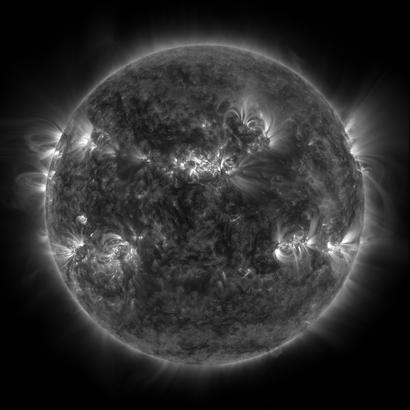
\includegraphics[width=0.3\columnwidth]{Figs/soleil_date_0.jpg}&
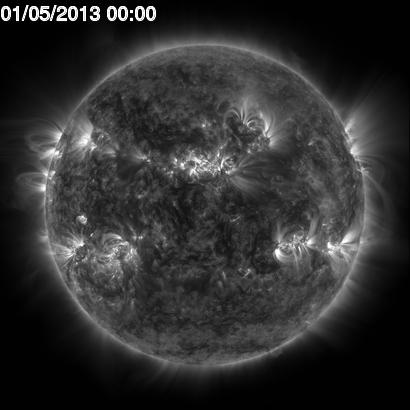
\includegraphics[width=0.3\columnwidth]{Figs/soleil_date_1.jpg}
\end{tabular}
\caption{\label{fig:soleil_date} Image avant et après incrustation de la date}
\end{figure}

Ce travail de réécriture peut être fait à l'aide de \sed en plusieurs étapes en passant par les réécritures suivantes~:
\begin{itemize}
\item[] 2012\_08\_31\_\_00\_00\_23\_34\_\_SDO\_AIA\_AIA\_211.jpg  (1)
\item[->] 2012\_08\_31\_\_00\_00 (2)
\item[->] 2012\_08\_31 00\_00 (3)
\item[->] 01/05/2013 00:00 (4)
\end{itemize}
Le passage de (1) à (2) peut se faire en supprimant (i.e. remplacer par une chaîne vide) un motif de la forme ``\_dd...d\_dd...d\_\_SDO\_AIA\_dd...d'' o{\`u} ``dd...d'' indique une séquence de longueur arbitraire de chiffre entre 0 et 9. Le motif pour caractériser un nombre arbitraire de chiffres entre 0 et 9 est "[0-9]*". Le passage de l'étape (2) à l'étape (3) se fait en remplaçant le motif "\_\_" par " ". Le passage de (3) à (4) peut se faire facilement en utilisant la capture de groupe. Prenons un exemple~:
\begin{exempleResultat}
bash:\$ echo 2012_08_31 | sed -r 's/([0-9]*)\_([0-9]*)\_([0-9]*)/\textbackslash{}3:\textbackslash{}2:\textbackslash{}1/'
01:05:2013
bash:\$ echo 2012_08_31 | sed -r 's/([0-9]*)\_([0-9]*)\_([0-9]*)/\textbackslash{}3\textbackslash{}/\textbackslash{}2\textbackslash{}/\textbackslash{}1/'
01/05/2013
\end{exempleResultat}
On remarquera l'utilisation de l'option "-r" qui permet d'utiliser des expressions régulières étendues (par opposition aux expressions régulières de base) et facilite l'écriture de l'expression régulière pour des groupes, c'est à dire les parties de l'expression de la forme "([0-9]*)". Si nous voulions utiliser les expressions régulières de base, nous aurions dû l'écrire "\textbackslash{}([0-9]*\textbackslash{})". \\

Nous sommes maintenant capables de constuire la chaîne de caractères à insérer sur l'image. Il reste ... à l'insérer. Pour cela, on peut utiliser \convert et son "-draw". Vous pouvez tester les commandes ci-dessous sur une image redimensionnée qu'on appellera img.jpg~:
\begin{exempleResultat}
bash:\$ convert img.jpg -fill white -draw "text 0,20 'Un super texte'" res.jpg 
bash:\$ convert img.jpg -pointsize 20 -fill white -draw "text 0,20 'Un super texte'" res.jpg 
\end{exempleResultat}

Vous pouvez maintenant intégrer les deux éléments précédents dans un script \bash{scripts/ecrit\_date.sh} qui prend des chemins d'image dans l'entrée standard, et utilise convert et sed pour incruster la date et l'heure dans l'image et sauvegarder les résultats dans le répertoire \bash{postproc\_images}.\\

Il reste une dernière chose à faire dans votre script \bash{scripts/ecrit\_date.sh}. Quand nous allons regrouper les images pour en former une vidéo, il faut que les images portent des noms de fichier qui soient des nombres consécutifs, ie 00000.jpg, 00001.jpg, ... ; On peut facilement l'ajouter dans le script Bash, en utilisant un compteur incrémenté à chaque fois qu'une image est traitée et utiliser la valeur de ce compteur pour construire le nom du fichier cible. Par exemple~:
\begin{exempleResultat}
bash:\$ count=0
bash:\$ echo {\$}count
0
bash:\$ count=`expr {\$}count + 1`
bash:\$ echo {\$}count
1
\end{exempleResultat}
Vous pouvez terminer votre script en affichant dans la sortie standard le nom du fichier généré. Sachez néanmoins que notre pipeline s'arrête là. La dernière étape qui consiste à créer une vidéo à partir des images se fait une fois que tout le pipeline précédent est terminé.\\

Ajoutez l'appel à votre script \bash{scripts/ecrit\_date.sh} dans le script \bash{all.sh}.

\subsection{Et finalement, la vidéo}

Il nous reste à voir une dernière chose: comment fabriquer une vidéo à partir d'une collection d'images? En arrivant à cette partie, vous devez déjà disposer d'un script \bash{all.sh} qui, lorsqu'il est exécuté, produit une séquence d'images numérotées successivement dans le répertoire \bash{postproc\_images}, à la bonne taille, au format jpg, et dans lesquelles la date et l'heure sont incrustées.\\

De manière générale, pour produire une vidéo à partir d'une séquence d'images numérotées successivement, il existe plusieurs outils, notamment \mencoder, \ffmpeg, \avconv. Nous allons ici utiliser \ffmpeg\footnote{on notera que avconv doit succéder à \ffmpeg mais qu'à l'heure o{\`u} ce TP est écrit, il est encore instable.}.  La façon la plus simple de générer une vidéo à partir d'une collection d'images JPEG est d'appeler la commande ci-dessous~:
\begin{center}
\bash{ffmpeg -i mesimages/\%05d.jpg mavideo.mp4}
\end{center}
J'ai ici supposé que les images étaient numérotées sur 5 chiffres, c'est ce qu'indique le format \%05d, i.e. un nombre sur 5 chiffres éventuellement précédés de 0.\\

La vidéo ainsi générée peut paraître lente. C'est dû à ce qu'on appelle le \emph{frame rate}, i.e. combien d'images sont affichées par seconde. Sachant que nous disposons d'environ 2500 images pour une journée. Si on souhaite que le film ne dure que 10 secondes, il va falloir utiliser une vitesse de lecture des images de 250 images par secondes. On peut changer la vitesse de lecture de la séquence d'images en précédant l'option "-i" par une option "-r" comme suit~:
\begin{center}
\bash{ffmpeg -r 250 -i mesimages/\%05d.jpg mavideo.mp4}
\end{center}
Enfin, si on veut garantir que les images ne soient pas compressées avant d'être ajoutées au film, on peut préciser à ffmpeg l'option "-qscale 1", ce qui donne finalement~:
\begin{center}
\bash{ffmpeg -qscale 1 -r 250 -i mesimages/\%05d.jpg mavideo.mp4}
\end{center}

Pour visualiser la vidéo, vous pouvez faire appel à \mplayer~:
\begin{center}
\bash{\mplayer mavideo.mp4}
\end{center}


\begin{center}
\colorbox{lblue}{\begin{minipage}{\linewidth}

\includegraphics[width=0.05\columnwidth]{Figs/warning.png}
\includegraphics[width=0.05\columnwidth]{Figs/warning.png}
\includegraphics[width=0.05\columnwidth]{Figs/warning.png}
\textbf{Super important}: N'oubliez pas de faire le ménage sur votre compte en enlevant notamment les images dans les répertoires raw\_images, images et postproc\_images, sinon on va se faire gronder pour utilisation abusive de l'espace disque.
\end{minipage}}
\end{center}

\subsection{En bonus: appliquer des fausses couleurs}

Jusqu'à maintenant, nous avons utilisé des images noir et blanc. Simplement, la vidéo est beaucoup plus sympa si nous lui appliquons des fausses couleurs. Pour appliquer des fausses couleurs, une façon de faire est de se construire un gradient de couleur qui sera indéxé par la luminance de l'image. On peut par exemple créer un gradient sous gimp, ci-dessous une image 600x30 avec un dégradé ``incandescent'' et un décalage de 35.
\begin{center}

\includegraphics[width=0.7\linewidth]{Figs/soleil_gradient.jpg}
\end{center}

L'application du gradient sur l'image noir et blanc peut alors se faire grâce à imagemagick. Imagemagick sait en effet utiliser des tables de conversion de couleur~:\url{http://www.imagemagick.org/Usage/color_mods/#color_lut}
\begin{center}
\bash{\convert src.jpg -colorspace gray gradient.jpg -clut out.jpg}
\end{center}
Ce qui nous donne~:
\begin{figure}[htbp]
\begin{tabular}{cc}
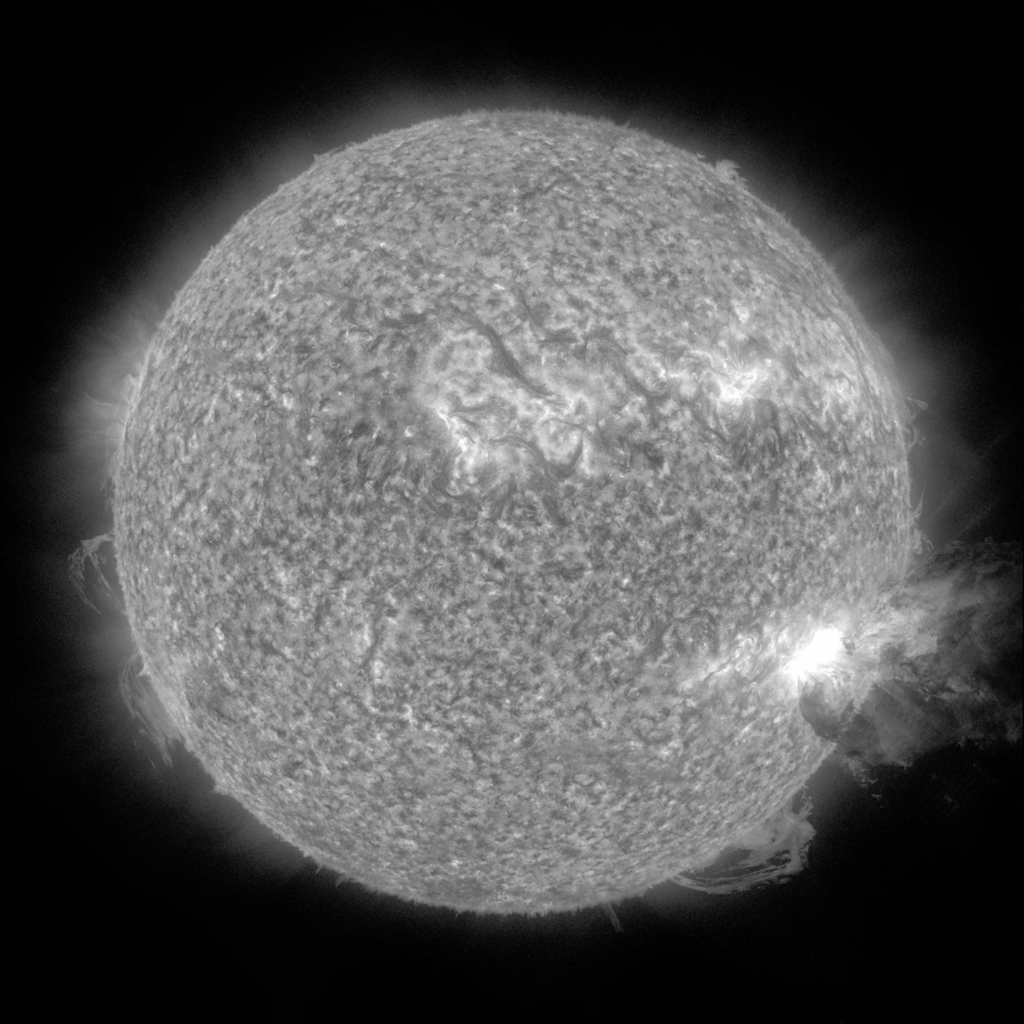
\includegraphics[width=0.3\columnwidth]{Figs/soleil_greyscale.jpg}&
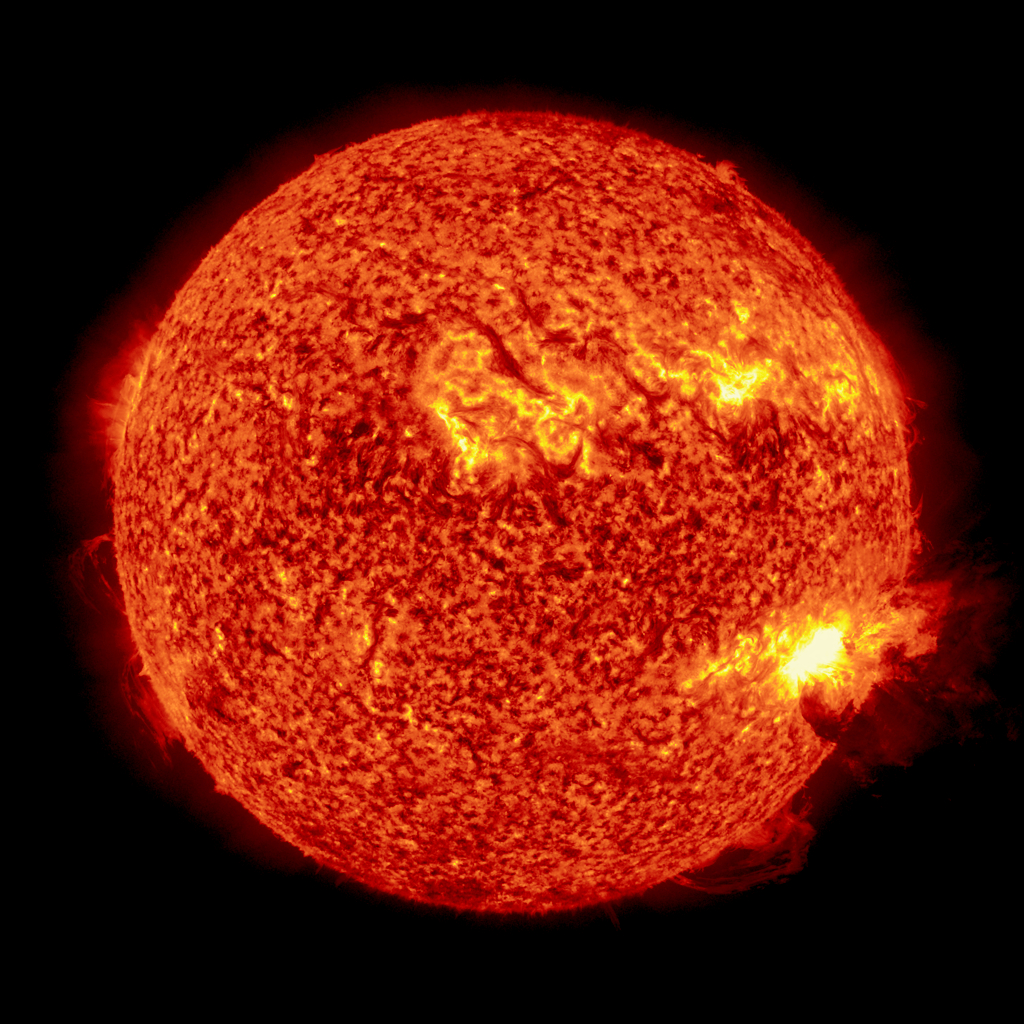
\includegraphics[width=0.3\columnwidth]{Figs/soleil_false_color.jpg}
\end{tabular}
\caption{\label{fig:soleil_false_color} Image avant et après colorisation.}
\end{figure}


\subsection{Notes d'installation pour refaire le TP chez vous}

Si vous voulez refaire ce TP chez vous, vous devez installer certains paquets qui ne sont pas installés par défaut. Sous Fedora, vous devez exécuter "su -c 'yum install -y ffmpeg ImageMagick mplayer'" en ayant au préalable installé les dépots rpmfusion \url{http://rpmfusion.org/}. Sous Ubuntu, "sudo apt-get install ffmpeg imagemagick mplayer" devrait faire l'affaire.


\vfill
\newpage
